\begin{Exercise}[title=Single neuron properties]
In this exercise we will take a look at a single neuron and it's properties.


\Question{Create a single neuron.}
Create an empty canvas by pressing the menu button in the upper left corner, then press select simulation and click on the empty canvas.

Press the grey arrow in the upper right corner to open the menu for adding new items. From left to right the upper row of menu items are: exitatory neurons, inhibitory neurons, measuring devices, generators and sensory input. 
Under the exitatory neuron menu you have, passive neurons, bursting neurons and adaptive neurons. It is similar for inhibitory neurons. Drag and drop a passive exitatory neuron onto the canvas. 

\begin{center}
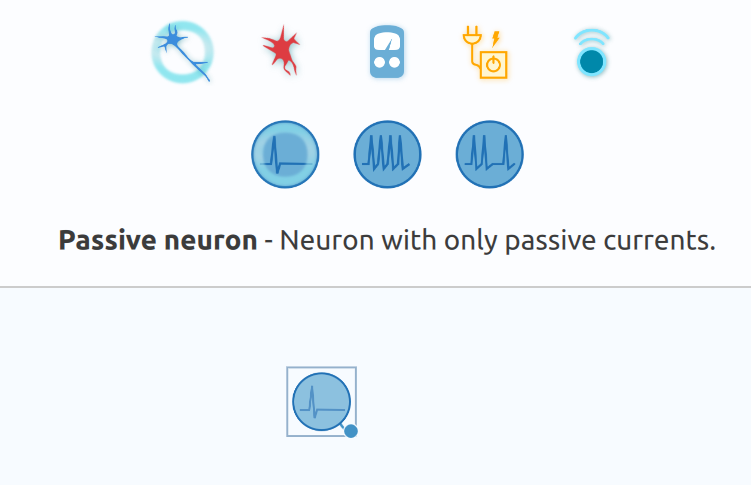
\includegraphics[width=10cm]{single_neuron.png}
\end{center}


\Question{Connect a voltmeter to the neuron.}

Under measuring devices you will find voltmeter and speaker. Drag and drop a voltmeter onto the canvas, then click the neuron and drag a connection to the voltmeter. The voltmeter will now the display the voltage from the neuron. The graph is flat because the neuron has no input yet.

\begin{center}
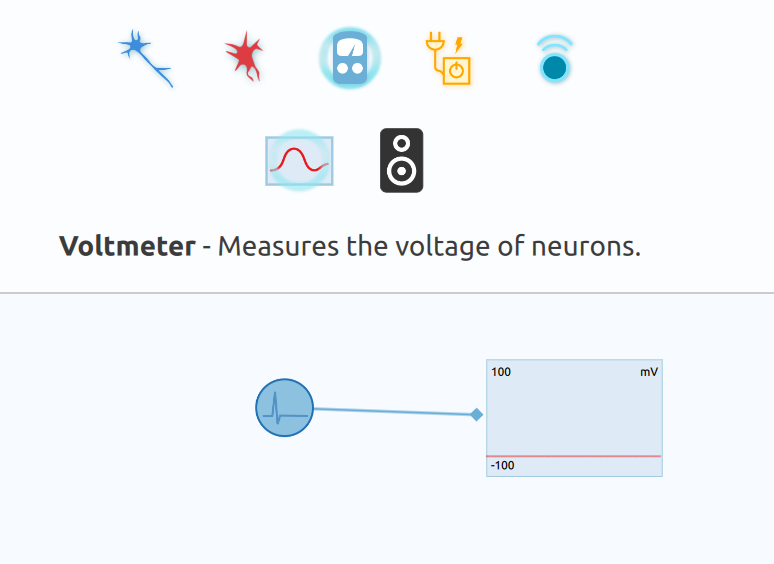
\includegraphics[width=10cm]{voltmeter.png}
\end{center}


\Question{Connect a DC generator to the neuron.}

Under generators you have DC clamp (straight arrow), AC clamp (wavy arrow) and Poisson generator (random noise, question mark). Drag the DC clamp onto the canvas and connect it to the neuron as we did with the voltmeter.


\begin{center}
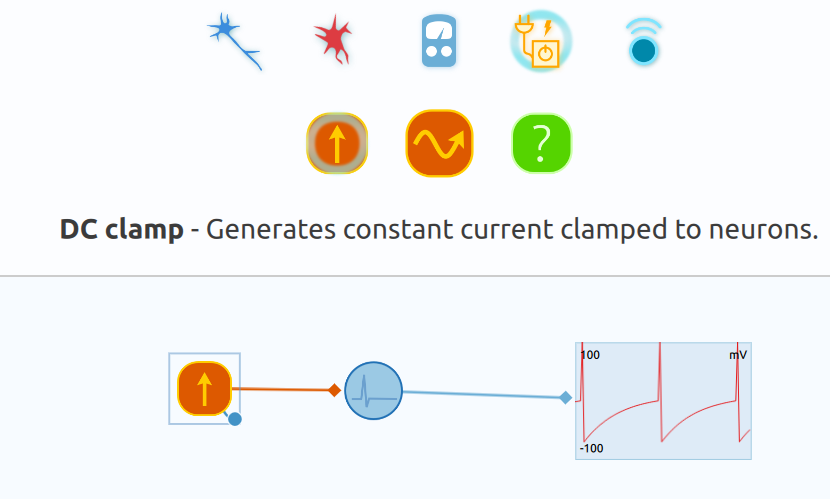
\includegraphics[width=10cm]{acgenerator.png}
\end{center}

We now have a single neuron that recieves input and generates spikes.

\Question{Play around with this setup.}

If you click on one of the three items that we have created and then press the gear in the lower left corner, you get the options menu for that specific item. Go through the DC clamp, exitatory neuron and voltmeter and change the settings to see what happens.

\Question{Expand this setup.}

%You should now have a understanding for how the different parameters influence this setup. 
Replace the DC clamp with the other input types (AC clamp, Poisson generator, etc.). Test different parameters for each of the input types to see how this affects the response of the neuron.

% \begin{itemize}
% \item Replace the DC generator with a AC generator
% \item Replace the DC generator with a Poisson generator
% \item Add a speaker to the neuron
% \item Use a touch sensor instead of a generator
% \item Use both a DC generator and a Poisson generator
% \item Use both a AC generator and a Poisson generator
% \end{itemize}


\end{Exercise}
